\documentclass[journal,12pt,twocolumn]{IEEEtran}

\usepackage{setspace}
\usepackage{textcomp}
\usepackage{gensymb}
\usepackage{xcolor}
\usepackage{caption}
\singlespacing
\usepackage[cmex10]{amsmath}
\usepackage{mathtools}
\usepackage{hyperref}
\usepackage{amsthm}
\usepackage{mathrsfs}
\usepackage{txfonts}
\usepackage{stfloats}
\usepackage{cite}
\usepackage{cases}
\usepackage{subfig}
\usepackage{longtable}
\usepackage{multirow}
\usepackage{enumitem}
\usepackage{mathtools}
\usepackage{listings}
\usepackage{tikz}
\let\vec\mathbf

% Tikz, Circuitikz
\usepackage{circuitikz}

\DeclareMathOperator*{\Res}{Res}
\renewcommand\thesection{\arabic{section}}
\renewcommand\thesubsection{\thesection.\arabic{subsection}}
\renewcommand\thesubsubsection{\thesubsection.\arabic{subsubsection}}

\renewcommand\thesectiondis{\arabic{section}}
\renewcommand\thesubsectiondis{\thesectiondis.\arabic{subsection}}
\renewcommand\thesubsubsectiondis{\thesubsectiondis.\arabic{subsubsection}}
\hyphenation{op-tical net-works semi-conduc-tor}

\lstset{
language=Python,
frame=single, 
breaklines=true,
columns=fullflexible
}

\begin{document}
%

\theoremstyle{definition}
\newtheorem{theorem}{Theorem}[section]
\newtheorem{problem}{Problem}
\newtheorem{proposition}{Proposition}[section]
\newtheorem{lemma}{Lemma}[section]
\newtheorem{corollary}[theorem]{Corollary}
\newtheorem{example}{Example}[section]
\newtheorem{definition}{Definition}[section]
\newcommand{\BEQA}{\begin{eqnarray}}
\newcommand{\EEQA}{\end{eqnarray}}
\newcommand{\define}{\stackrel{\triangle}{=}}
\newcommand{\myvec}[1]{\ensuremath{\begin{pmatrix}#1\end{pmatrix}}}
\newcommand{\mydet}[1]{\ensuremath{\begin{vmatrix}#1\end{vmatrix}}}

\bibliographystyle{IEEEtran}

\providecommand{\nCr}[2]{\,^{#1}C_{#2}} % nCr
\providecommand{\nPr}[2]{\,^{#1}P_{#2}} % nPr
\providecommand{\mbf}{\mathbf}
\providecommand{\pr}[1]{\ensuremath{\Pr\left(#1\right)}}
\providecommand{\qfunc}[1]{\ensuremath{Q\left(#1\right)}}
\providecommand{\sbrak}[1]{\ensuremath{{}\left[#1\right]}}
\providecommand{\lsbrak}[1]{\ensuremath{{}\left[#1\right.}}
\providecommand{\rsbrak}[1]{\ensuremath{{}\left.#1\right]}}
\providecommand{\brak}[1]{\ensuremath{\left(#1\right)}}
\providecommand{\lbrak}[1]{\ensuremath{\left(#1\right.}}
\providecommand{\rbrak}[1]{\ensuremath{\left.#1\right)}}
\providecommand{\cbrak}[1]{\ensuremath{\left\{#1\right\}}}
\providecommand{\lcbrak}[1]{\ensuremath{\left\{#1\right.}}
\providecommand{\rcbrak}[1]{\ensuremath{\left.#1\right\}}}
\theoremstyle{remark}
\newtheorem{rem}{Remark}
\newcommand{\sgn}{\mathop{\mathrm{sgn}}}
\providecommand{\abs}[1]{\left\vert#1\right\vert}
\providecommand{\res}[1]{\Res\displaylimits_{#1}} 
\providecommand{\norm}[1]{\lVert#1\rVert}
\providecommand{\mtx}[1]{\mathbf{#1}}
\providecommand{\mean}[1]{E\left[ #1 \right]}
\providecommand{\fourier}{\overset{\mathcal{F}}{ \rightleftharpoons}}
\providecommand{\ztrans}{\overset{\mathcal{Z}}{ \rightleftharpoons}}
\providecommand{\laplace}{\overset{\mathcal{L}}{ \longrightarrow}}
\providecommand{\system}{\overset{\mathcal{H}}{ \longleftrightarrow}}
\newcommand{\solution}{\noindent \textbf{Solution: }}
\providecommand{\dec}[2]{\ensuremath{\overset{#1}{\underset{#2}{\gtrless}}}}
\numberwithin{equation}{section}
\makeatletter
\@addtoreset{figure}{problem}
\makeatother

\let\StandardTheFigure\thefigure
\renewcommand{\thefigure}{\theproblem}

\def\putbox#1#2#3{\makebox[0in][l]{\makebox[#1][l]{}\raisebox{\baselineskip}[0in][0in]{\raisebox{#2}[0in][0in]{#3}}}}
     \def\rightbox#1{\makebox[0in][r]{#1}}
     \def\centbox#1{\makebox[0in]{#1}}
     \def\topbox#1{\raisebox{-\baselineskip}[0in][0in]{#1}}
     \def\midbox#1{\raisebox{-0.5\baselineskip}[0in][0in]{#1}}

\vspace{3cm}

\title{ Circuits and Transforms }
\author{ Sumanth N R }
\maketitle
\tableofcontents

\renewcommand{\thefigure}{\theenumi}
\renewcommand{\thetable}{\theenumi}

\bigskip

\begin{abstract}
This manual provides a simple introduction to Transforms
\end{abstract}


\section{Definitions}

\begin{enumerate}[label=\arabic*.,ref=\thesection.\theenumi]
\numberwithin{equation}{section}
\numberwithin{figure}{section}

\item The unit step function is 
	\begin{align} u(t) = \begin{cases}
		1 & t > 0 \\
		\frac{1}{2} & t = 0 \\
		0 & t < 0
	\end{cases} \end{align}

\item The Laplace transform of $g(t)$ is defined as 
	\begin{align}
		G(s) = \int_{-\infty}^{\infty} g(t) e^{-st}\, dt
	\end{align}

\end{enumerate}



\section{Laplace Transform}

\begin{enumerate}[label=\arabic*.,ref=\thesection.\theenumi]
\numberwithin{equation}{section}

\item
	In the circuit, the switch S is connected to position P for a long time so that the charge on the capacitor becomes $q_1 \, \mu C$. Then S is switched to position Q.  After a long time, the charge on the capacitor is
	$q_2 \, \mu C$.
	\begin{figure}[!ht]
		\centering
		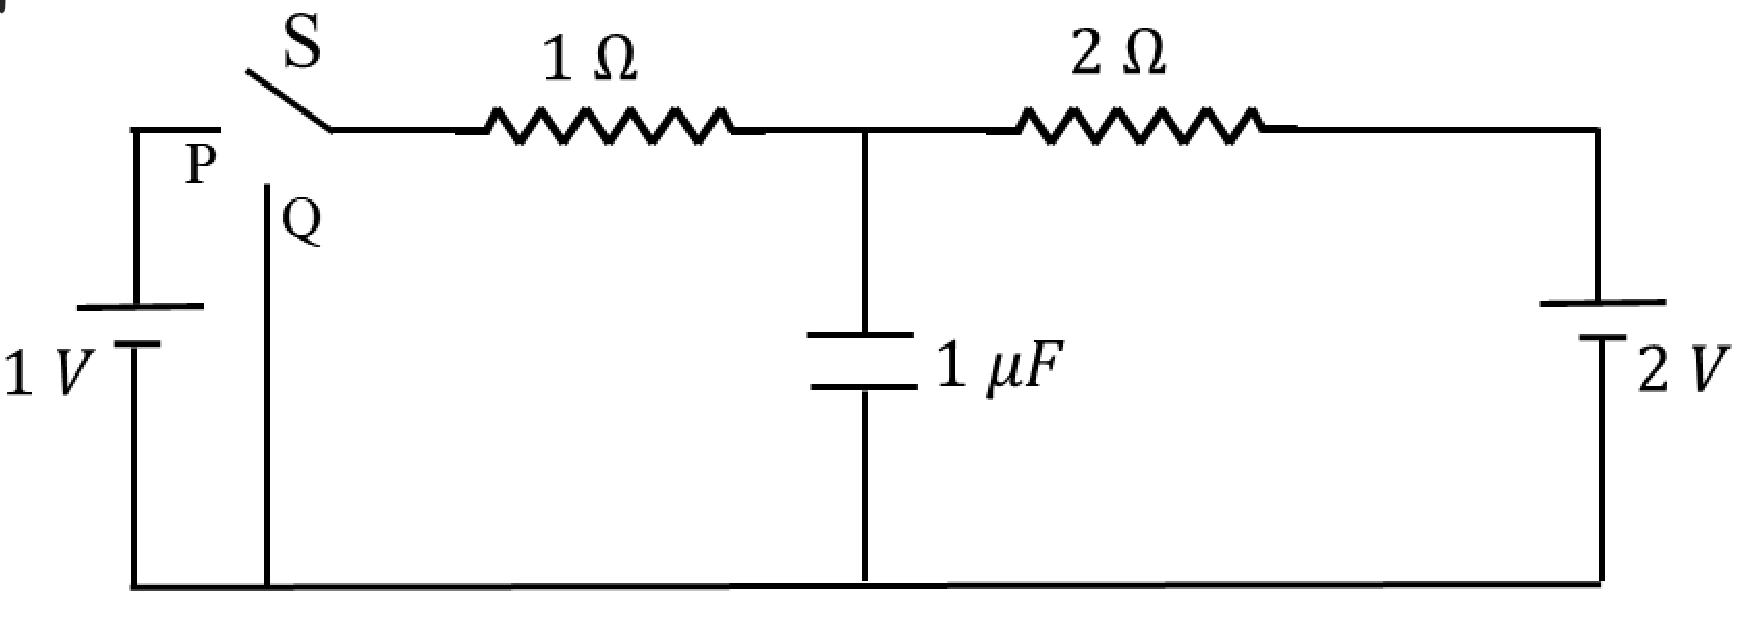
\includegraphics[width=\columnwidth]{figs/ckt.jpg}
		\caption{}
		\label{fig:ckt}
	\end{figure}


\item Draw the circuit using latex-tikz. \\
	\solution\\
	\begin{circuitikz}[scale=0.7] \draw
		(0, 0) to [short] (10, 0)
		(5, 0) to [C=1$\mu$F] (5, 3)
		(10, 3) to [battery1, l=2V] (10, 0)
		(5, 3) to [R=2$\ohm$] (10, 3)
		(0, 3) to [short] (1, 3)
		(1, 3) to [nos, invert] (2, 3)
		(2, 3) to [R=1$\ohm$] (5, 3)
		(1, 0) to [short] (1, 2.75)
		(0, 0) to [battery1, l=1V, invert] (0, 3)
		(0.75, 3) node[label={above:P}] {}
		(2, 3) node[label={above:S}] {}
		(1, 2.5) node[label={right:Q}] {}
		;
	\end{circuitikz}


\item Find $q_1$. \\
	\solution\\
	Current through the capacitor is $0$ at steady state. So, current only flows in the outer loop.\\
	\begin{circuitikz}[scale=0.6] \draw
		(0, 0) to [short] (10, 0)
		(5, 3) to [R=$2\ohm$] (10, 3)
		(0, 3) to [R=$1\ohm$] (5, 3)
		(10, 3) to [battery1, l=$2V$, i<=$i$] (10, 0)
		(0, 0) to [battery1, l=$1V$, invert] (0, 3)
		;
	\end{circuitikz}
	\begin{align*}
    	i &= \frac{(2 - 1)\ V}{(1 + 2)\ \ohm} \\
    	i &= \frac{1}{3} A
	\end{align*}
	Potential difference across the capacitor, 
	\begin{align*}
		V_C &= 2 - 2 \times \frac{1}{3} = \frac{4}{3} V \\
		q_1 &= C V_C \\
		q_1 &= 1 \mu F \times \frac{4}{3} V \\
		q_1 &= \frac{4}{3} \mu C
	\end{align*}


\item Show that the Laplace transform of $u(t)$ is $\frac{1}{s}$ and find the ROC.\\
	\solution\\
	By the definition of Laplace transform
	\begin{align*}
		u(t) \laplace & \int_{-\infty}^\infty u(t) e^{-st} dt 
			= \int_0^\infty e^{-st} dt \\
			=& \left. \frac{e^{-st}}{-s} \right|_0^\infty = \frac{1}{s}
	\end{align*}
	$\lim_{s \to \infty} e^{-st} = 0$ only when $Re(s) > 0$. \\
	The ROC is $Re(s) > 0$.


\item Show that 
	\begin{align}
		e^{-at}u(t) \system{L} \frac{1}{s+a}, \quad a > 0
	\end{align}
	and find the ROC.\\
	\solution\\
	By the definition of Laplace transform
	\begin{align*}
		e^{-at}u(t) \laplace & \int_{-\infty}^\infty e^{-at}u(t) e^{-st} dt \\
			=& \int_0^\infty e^{-(s+a)t} dt \\
			=& \left. \frac{e^{-(s+a)t}}{-(s+a)} \right|_0^\infty = \frac{1}{s+a}
	\end{align*}
	$\lim_{s \to \infty} e^{-(s+a)t} = 0$ only when $Re(s+a) > 0$. \\
	The ROC is $Re(s+a) > 0$ or $Re(s) > -a$.



\item Now consider the following resistive circuit transformed from 
	Fig. \ref{fig:ckt}
	\begin{figure}[!ht]
		\centering
		% 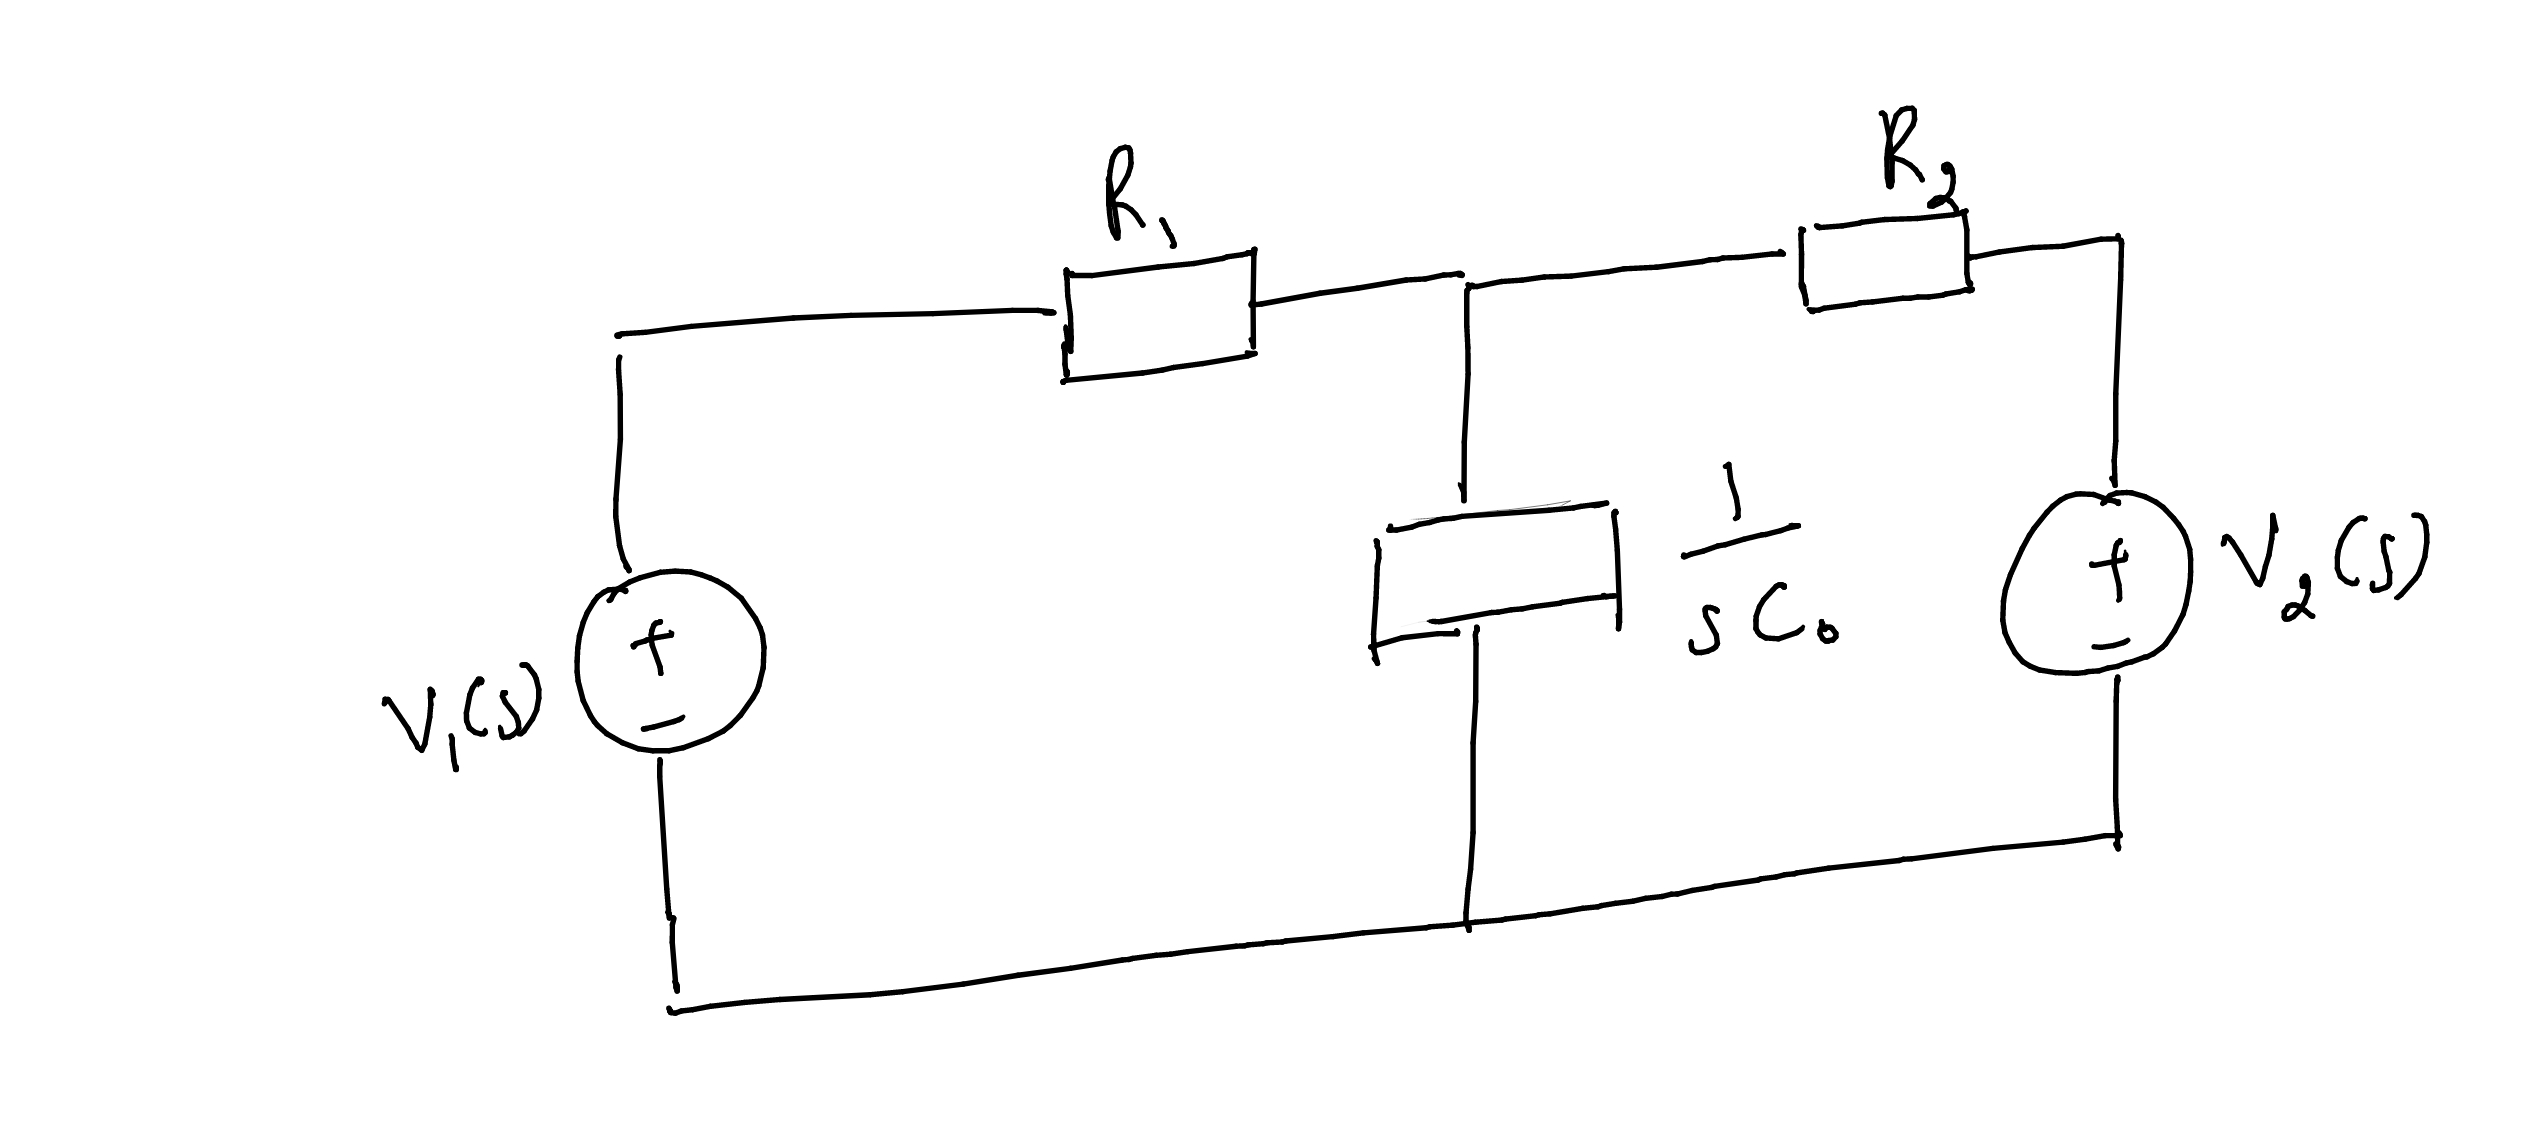
\includegraphics[width=\columnwidth]{figs/lap-ckt.jpg}
		\begin{circuitikz}[scale=0.6] \draw
		(0, 0) to [short] (10, 0)
		(5, 0) to [C=$\frac{1}{sC_0}$, i<=$I_1(s)$] (5, 3)
		(5, 3) to [R=$R_2$] (10, 3)
		(0, 3) to [R=$R_1$, i<=$I_2(s)$] (5, 3)
		(10, 3) to [battery1, l=$\frac{V_2}{s}$, i<=$I(s)$] (10, 0)
		(0, 0) to [battery1, l=$\frac{V_1}{s}$, invert] (0, 3)
		;
		\end{circuitikz}

		\caption{}
		\label{fig:lap-ckt}
	\end{figure}
	where 
	\begin{align}
		u(t) \system{L} V_1(s) \\
		2u(t) \system{L} V_2(s)
	\end{align}
	Find the voltage across the capacitor $V_{C_0}(s)$.

	\solution\\
	Using the Transform from time domain to s-domain
	\begin{align*}
		V_1(s) &= \mathcal{L}(u(t)) = \frac{V_1}{s} \\
		V_2(s) &= \mathcal{L}(2u(t)) = \frac{V_2}{s}
	\end{align*}

	Potential across the capacitor is $V_{C_0}(s)$ and the assuming bottom is grounded. \\
	Applying KCL at the upper junction, we have,
	\begin{align*}
		&\frac{V_{C_0}(s) - V_1(s)}{R_1} + \frac{V_{C_0}(s) - V_2(s)}{R_2} + \frac{V_{C_0}(s)}{\frac{1}{s C_0}} = 0 \\
		&V_{C_0}(s) \brak{\frac{1}{R_1} + \frac{1}{R_2} + s C_0} = \frac{V_1(s)}{R_1} + \frac{V_2(s)}{R_2} \\
		&V_{C_0}(s) = \frac{V_1(s)R_2 + V_2(s)R_1}{R_1 + R_2 + s C_0 R_1 R_2} \\
		&V_{C_0}(s) = \frac{R_2 + 2R_1}{s(R_1 + R_2 + s C_0 R_1 R_2)} 
	\end{align*}
	after substitution.


\item Find $v_{C_0}(t)$.  Plot using python.\\
	\solution\\
	Factoring $V_{C_0}(s)$, we have 
	\begin{align*}
		&V_{C_0}(s) = \left( \frac{1}{R_1+R_2} \right) \left( \frac{\brak{R_2 + 2R_1}}{s} - \frac{R_1 R_2 C_0 \brak{R_2 + 2R_1}}{R_1 + R_2 + sC_0 R_1 R_2} \right) \\
		&= \brak{\frac{R_2 + 2R_1}{R_1 + R_2}} \brak{\frac{1}{s} - \frac{R_1 R_2 C_0}{R_1 + R_2 + sC_0 R_1 R_2}} \\
		&= \brak{\frac{R_2 + 2R_1}{R_1 + R_2}} \brak{\frac{1}{s} - \frac{1}{\frac{1}{R_2 C_0} + \frac{1}{R_1 C_0} + s}} 
	\end{align*}
	Applying inverse Laplace transform,
	\begin{align}
		v_{C_0}(t) = \frac{R_2 + 2R_1}{R_1 + R_2} \brak{u(t) - e^{-\brak{\frac{1}{R_1 C_0} + \frac{1}{R_2 C_0}} \, t} u(t)}
		\label{eq:vC0}
	\end{align}
	Using the values $R_1 = 1 \, \Omega$, $R_2 = 2 \, \Omega$, $C_0 = 1 \, \mu F$, we get
	\begin{align*}
		v_{C_0}(t) = \frac{4}{3} u(t) \brak{1 - e^{-1.5 \times 10^{6} \, t}} 
	\end{align*}
	The following code yields $v_{C_0}(t)$.
	\begin{lstlisting}
wget https://github.com/Sigma1084/EE3900/blob/master/cktsig/code/Ex2_plotVt.py
	\end{lstlisting}
	\begin{figure}[!ht]
		\centering
		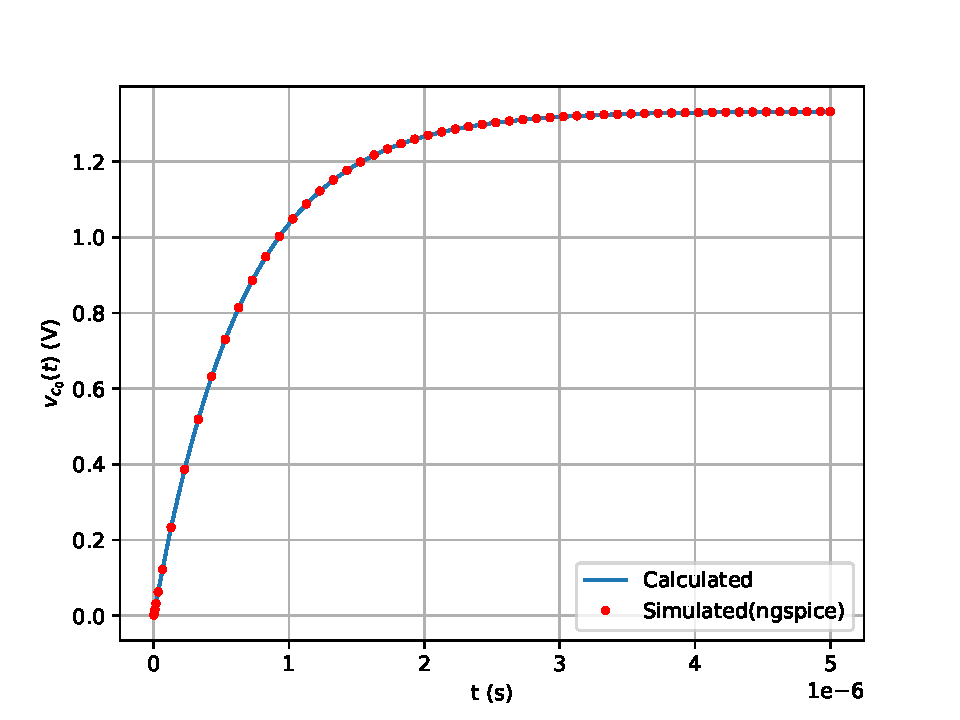
\includegraphics[width=\columnwidth]{figs/Ex2_vt.pdf}
		\caption {}
		\label{fig:vt_calc}
	\end{figure}
	\pagebreak


\item Verify your result using ngspice.
	The following code yields $v_{C_0}(t)$. using ngspice
	\begin{lstlisting}
wget https://github.com/Sigma1084/EE3900/blob/master/cktsig/code/Ex2.spice
	\end{lstlisting}



\item Obtain Fig. \ref{fig:lap-ckt} using the equivalent differential equation. \\
	\solution\\
	\begin{circuitikz}[scale=0.6] \draw
		(0, 0) to [short] (10, 0)
		(5, 0) to [C=$C_0$, i<=$i_1$] (5, 3)
		(5, 3) to [R=$R_2$] (10, 3)
		(0, 3) to [R=$R_1$, i<=$i_2$] (5, 3)
		(10, 3) to [battery1, l=$V_2$, i<=$i$] (10, 0)
		(0, 0) to [battery1, l=$V_1$, invert] (0, 3)
		;
	\end{circuitikz}
	Using KVL on the left and right loops, we get
	\begin{align}
		i_2(t) \ R_1 + V_1 - \int_0^t \frac{i_1(t)}{C_0} dt &= 0 \label{eq:q2_diff} \\
		-i(t) \ R_2 + V_2 - \int_0^t \frac{i_1(t)}{C_0} dt &= 0
	\end{align}
	Taking the Laplace Transform after multiplying u(t) in both equations,
	\begin{align*}
		\mathcal{L} \left( R_1 i_2(t)u(t) + V_1u(t) - u(t)\int_0^t \frac{i_1}{C_0} dt \right) &= 0 \\
		\mathcal{L} \left( -R_2 i(t)u(t) + V_2u(t) - u(t)\int_0^t \frac{i_1}{C_0} dt \right) &= 0
	\end{align*}
	Suppose $i(t)u(t) \laplace I(s) \text{ and } Vu(t) \laplace \frac{V}{s}$
	\[
		\implies \mathcal{L} \left( u(t) \int_0^t \frac{i_1}{C_0} dt \right)
		= \frac{1}{sC_0} \mathcal{L} \left( u(t)i_1 \right)
		= \frac{I_1(s)}{sC_0}
	\]
	(Using the properties of Laplace Transform) \\
	The above equations after transform
	\begin{align}
		R_1 I_2(s) + \frac{V_1}{s} - \frac{I_1(s)}{sC_0} &= 0 \label{eq:q2_diff_lap} \\
		-R_2 I(s) + \frac{V_2}{s} - \frac{I_1(s)}{sC_0} &= 0 
	\end{align}
	Now after applying the transformation, from time domain to s-domain, we replace the capacitor with an equivalent resistor of resistence $\frac{1}{sC_0}$ and replace $I$ by $I(s)$, $V$ by $\frac{V}{s}$
	
	The equivalent s-domain circuit is now,
	\begin{circuitikz}[scale=0.6] \draw
		(0, 0) to [short] (10, 0)
		(5, 0) to [C=$\frac{1}{sC_0}$, i<=$I_1(s)$] (5, 3)
		(5, 3) to [R=$R_2$] (10, 3)
		(0, 3) to [R=$R_1$, i<=$I_2(s)$] (5, 3)
		(10, 3) to [battery1, l=$\frac{V_2}{s}$, i<=$I(s)$] (10, 0)
		(0, 0) to [battery1, l=$\frac{V_1}{s}$, invert] (0, 3)
		;
	\end{circuitikz}


\end{enumerate}


\section{Initial Conditions}
\begin{enumerate}[label=\arabic*.,ref=\thesection.\theenumi]
\numberwithin{equation}{section}


\item Find $q_2$ in Fig. \ref{fig:ckt} \\
	\solution\\
	Current through the capacitor is $0$ in steady state. 
	Since the current flows only in the outer loop, let the current in the outer loop be $I$.
	\begin{align*}
		I = \frac{2V}{(1+2)\ohm} = \frac{2}{3}A
	\end{align*}
	So, the potential difference across the capacitor is
	\begin{align*}
		V_{C_0} &= 2 - \left( \frac{2}{3} \times 2 \right) = \frac{2}{3} V \\
		q_2 &= C V_{C_0} \\
		q_2 &= 1 \mu C \times \frac{2}{3} V \\
		q_2 &= \frac{2}{3} \mu C
	\end{align*}


\item Draw the equivalent $s$-domain resistive circuit when S is switched to position Q.  Use variables $R_1, R_2, C_0$ for the passive elements.
Use latex-tikz. \label{prob:init} \\
	\solution\\
	\begin{circuitikz}[american, scale=0.6] \draw
		(0, 0) to [short] (12, 0)
		(6, 2) to [C=$\frac{1}{sC_0}$] (6, 0)
		(6, 4) to [V,v=$\frac{V_0}{s}$] (6, 2)
		(6, 4) to [R=$R_2$] (12, 4)
		(0, 4) to [R=$R_1$] (6, 4)
		(12, 4) to [battery1, l=$\frac{V_2}{s}$] (12, 0)
		(0, 0) to [short] (0, 4)
		;
	\end{circuitikz}

	
\item $V_{C_0}(s)$ = ?\\
	\solution\\
	Applying KCL at the upper junction and assuming the bottom is grounded, we have,
	\begin{align*}
		&\frac{V_{C_0}(s) }{R_1} + \frac{V_{C_0}(s) - \frac{V_2}{s}}{R_2} + \frac{V_{C_0}(s) - \frac{V_0}{s}}{\frac{1}{s C_0}} = 0 \\
		&V_{C_0}(s) \brak{\frac{1}{R_1} + \frac{1}{R_2} + s C_0} = \frac{V_2}{sR_2} + V_0C_0 \\
		&V_{C_0}(s) = \frac{\frac{V_2}{sR_2} + V_0C_0} {\frac{1}{R_1} + \frac{1}{R_2} + s C_0}\\
		&V_{C_0}(s) = V_0\brak{\frac{1}{\frac{1}{C_0}\brak{\frac{1}{R_1} + \frac{1}{R_2}}+s}} \\
		&+ \frac{V_2}{R_2\brak{\frac{1}{R_1} +\frac{1}{R_2}}}\brak{\frac{1}{s} - \frac{1}{\frac{1}{C_0}\brak{\frac{1}{R_1} + \frac{1}{R_2}} + s}}
	\end{align*}
	

\item $v_{C_0}(t)$ = ? Plot using python.\\
	\solution\\
	Applying inverse Laplace transform to $V_{C_0}(s)$, we have,
	\begin{align*}
		&v_{C_0}(t) = V_0e^{-\brak{\frac{1}{R_1} + \frac{1}{R_2}}\frac{t}{C_0}}u(t) \nonumber \\ 
		&+ \frac{V_2}{R_2\brak{\frac{1}{R_1}+\frac{1}{R_2}}}\brak{1 - e^{-\brak{\frac{1}{R_1} + \frac{1}{R_2}}\frac{t}{C_0}}}u(t)
	\end{align*}
	Substituting the values $R_1=1, R_2=2, C_0=1\mu F, V_0=\frac{4}{3}V, V_2=2V$
	\begin{align}
		&v_{C_0}(t) = \frac{2}{3} \brak{1 + e^{-\brak{1.5 \times 10^6}t}}u(t)
		\label{eq:vc0t}
	\end{align}

	The following code yields $v_{C_0}(t)$.
	\begin{lstlisting}
wget https://github.com/Sigma1084/EE3900/blob/master/cktsig/code/Ex3_plotVt.py
	\end{lstlisting}

	\begin{figure}[!ht]
		\centering
		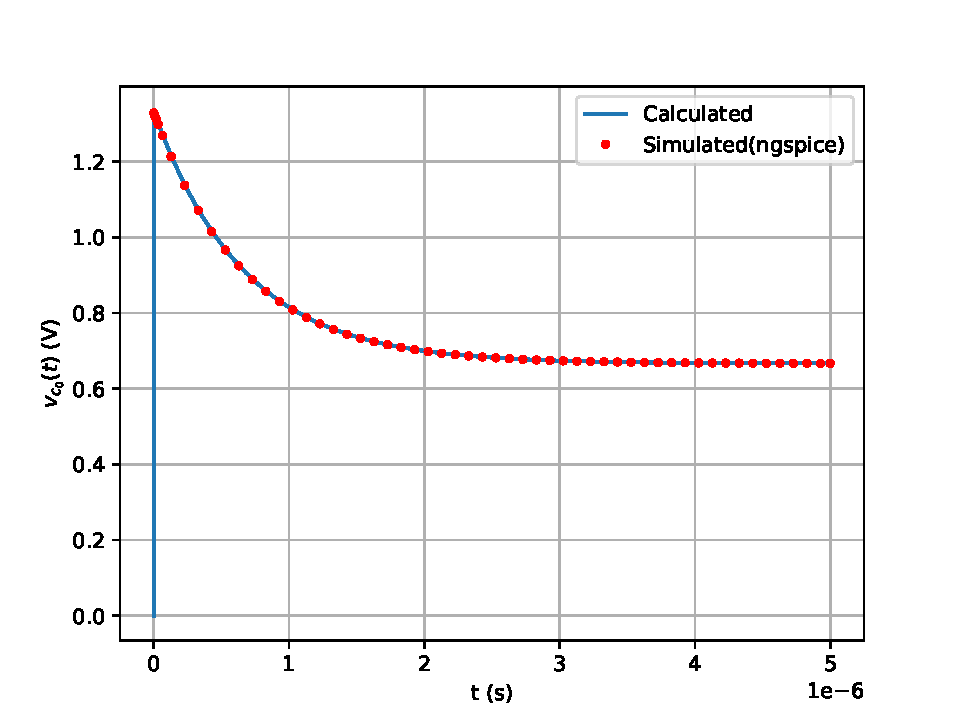
\includegraphics[width=\columnwidth]{figs/Ex3_vt.pdf}
		\caption {}
		\label{fig:q3_vc}
	\end{figure}


\item Verify your result using ngspice.
The following code yields $v_{C_0}(t)$. using ngspice
\begin{lstlisting}
wget https://github.com/Sigma1084/EE3900/blob/master/cktsig/code/Ex3.spice
\end{lstlisting}

	

\item Find $v_{C_0}(0-), v_{C_0}(0+)$ and  $v_{C_0}(\infty) $.\\
	\solution\\
	Using the initial conditions, we have,
	\begin{align*}
		v_{C_0}(0-) &= \frac{q_1}{C_0} = \frac{4}{3}V
	\end{align*}
	Using \eqref{eq:vc0t}, we have,
	\begin{align*}
		v_{C_0}(0+) &= \frac{2}{3} \brak{1 + e^{-\brak{1.5 \times 10^6}0}}u(0^+) = \frac{4}{3}V \\
		v_{C_0}(\infty) &= \frac{2}{3} \brak{1 + e^{-\brak{1.5 \times 10^6}\infty}}u(\infty) = \frac{2}{3}V
	\end{align*}
	

\item Obtain the Fig.  in problem \ref{prob:init} using the equivalent differential equation.\\
	\solution\\
	Constructing the circuit, \\
	\begin{circuitikz}[american, scale=0.6] \draw
		(0, 0) to [short] (12, 0)
		(6, 0) to [C=$C_0$, *-, i<=$i_1$] (6, 3)
		(6, 4.5) to [V,v=$V_0$] (6, 3)
		(6, 4.5) to [short] (6, 5)
		(6, 5) to [R=$R_2$] (12, 5)
		(0, 5) to [R=$R_1$, -*, i<=$i_2$] (6, 5)
		(12, 5) to [battery1, l=$V_2$, i=$i$] (12, 0)
		(0, 0) to [short] (0, 5)
		(6, 5) node[label={above:P}] {}
		(6, 0) node[label={below:Q}] {}
		;
	\end{circuitikz}
	Using KVL on both the left and outer loops, we have
	\begin{align*}
		-i_2(t) \ R_1 + V_0 + \int_0^t \frac{i_1(t)}{C_0} dt &= 0 \\
		-i(t) \ R_2 + V_2 - i_2(t) \ R_1 &= 0
	\end{align*}
	Taking the Laplace Transform after multiplying u(t) in both equations,
	\begin{align*}
		\mathcal{L} \left( -R_1 i_2(t)u(t) + V_0u(t) + u(t)\int_0^t \frac{i_1}{C_0} dt \right) &= 0 \\
		\mathcal{L} \left( -R_2 i(t)u(t) + V_2u(t) - R_1 i_2(t)u(t) \right) &= 0
	\end{align*}
	Suppose $i(t)u(t) \laplace I(s) \text{ and } Vu(t) \laplace \frac{V}{s}$
	\[
		\implies \mathcal{L} \left( u(t) \int_0^t \frac{i_1}{C_0} dt \right)
		= \frac{1}{sC_0} \mathcal{L} \left( u(t)i_1 \right)
		= \frac{I_1(s)}{sC_0}
	\]
	(Using the properties of Laplace Transform) \\
	The above equations after transform
	\begin{align*}
		R_1 I_2(s) + \frac{V_0}{s} + \frac{I_1(s)}{sC_0} &= 0\\
		-R_2 I(s) + \frac{V_2}{s} - R_1 I_2(s) &= 0 
	\end{align*}
	Now after applying the transformation, from time domain to s-domain, we replace the capacitor with an equivalent resistor of resistence $\frac{1}{sC_0}$ and replace $I$ by $I(s)$, $V$ by $\frac{V}{s}$, and hence we get,

	\begin{circuitikz}[american, scale=0.6] \draw
		(0, 0) to [short] (12, 0)
		(6, 0) to [C=$\frac{1}{sC_0}$, *-, i<=$I_1(s)$] (6, 3)
		(6, 4.5) to [V,v=$\frac{V_0}{s}$] (6, 3)
		(6, 4.5) to [short] (6, 5)
		(6, 5) to [R=$R_2$] (12, 5)
		(0, 5) to [R=$R_1$, -*, i<=$I_2(s)$] (6, 5)
		(12, 5) to [battery1, l=$\frac{V_2}{s}$, i=$I(s)$] (12, 0)
		(0, 0) to [short] (0, 5)
		(6, 5) node[label={above:P}] {}
		(6, 0) node[label={below:Q}] {}
		;
	\end{circuitikz}


\end{enumerate}


\section{Bilinear Transform}
\begin{enumerate}[label=\arabic*.,ref=\thesection.\theenumi]
\numberwithin{equation}{section}


\item In Fig. \ref{fig:ckt}, Consider the case when $S$ is switched to
	$Q$ right in the beginning. Formulate the differential equation. \\
	\solution\\
	Special Case of \eqref{eq:q2_diff}, putting $V_1 = 0$, we get
	\begin{align}
		i_2(t) \ R_1 - \int_0^t \frac{i_1(t)}{C_0} dt &= 0 \label{eq:q4_diff} \\
		-i(t) \ R_2 + V_2 - \int_0^t \frac{i_1(t)}{C_0} dt &= 0
	\end{align}
	The above equations after transformation to s-domain
	\begin{align}
		R_1 I_2(s) - \frac{I_1(s)}{sC_0} &= 0 \label{eq:q4_diff_lap} \\
		-R_2 I(s) + \frac{V_2}{s} - \frac{I_1(s)}{sC_0} &= 0 
	\end{align}


\item Find $H(s)$ considering the ouput voltage at the capacitor. \\
	\solution \\
	Recall that \( H(s) = \frac{V_{C_0}(s)}{V_2(s)} \) \\
	Using KCL at point P, after s-domain transform, we have,
	\[ \frac{V_{C_0}(s)}{R_1} + \frac{V_{C_0}(s)}{\frac{1}{sC_0}} + 
		\frac{V_{C_0}(s) - V_2(s)}{R_2} = 0 \]
	\[ V_{C_0}(s) \brak{\frac{1}{R_1} + sC_0 + \frac{1}{R_2}} = \frac{V_2(s)}{R_2} \]
	\[ \frac{V_{C_0}(s)}{V_2(s)} = H(s) = \frac{1}{R_2\brak{\frac{1}{R_1} +
		\frac{1}{R_2} + sC_0}} \]


\item Plot $H(s)$.  What kind of filter is it? \\
	\solution The following code yields the graph \\
	\begin{listing}

	\end{listing}
	Clearly, H(s) is a low pass filter
	

\item Using trapezoidal rule for integration, formulate the difference equation by considering
	\begin{align}
		y(n) = y(t)\vert_{t=n}
	\end{align}
	\solution \\



	\item Find $H(z)$.


	\item How can you obtain $H(z)$ from $H(s)$?
	

	\end{enumerate}
\end{document}


\end{document}
